\documentclass[12pt]{article}
\usepackage{graphicx}
\usepackage{graphics}
\usepackage{refstyle}
\usepackage{amsmath}
\usepackage{caption}
\usepackage{float}
\usepackage{booktabs}
\usepackage{array}
\usepackage{amssymb}
\usepackage{booktabs}
\let\vec\mathbf
\providecommand{\brak}[1]{\ensuremath{\left(#1\right)}}
\graphicspath{{/storage/self/primary/Download/latexnew/fig}}                                            
\graphicspath{{/storage/self/primary/Download/latexnew/table}}
\begin{document}
\title{\textbf{VECTOR}}
\date{}
\maketitle
\textbf{Question:} $\vec{P}$ and $\vec{Q}$ are any two points lying on the sides $DC$ and $AD$ respectively of a parallelogram $ABCD$.Show that, $ar\brak{\triangle APB}=ar\brak{\triangle BQC}$.


\textbf{Figure:}
\begin{figure}[H]
    \centering
   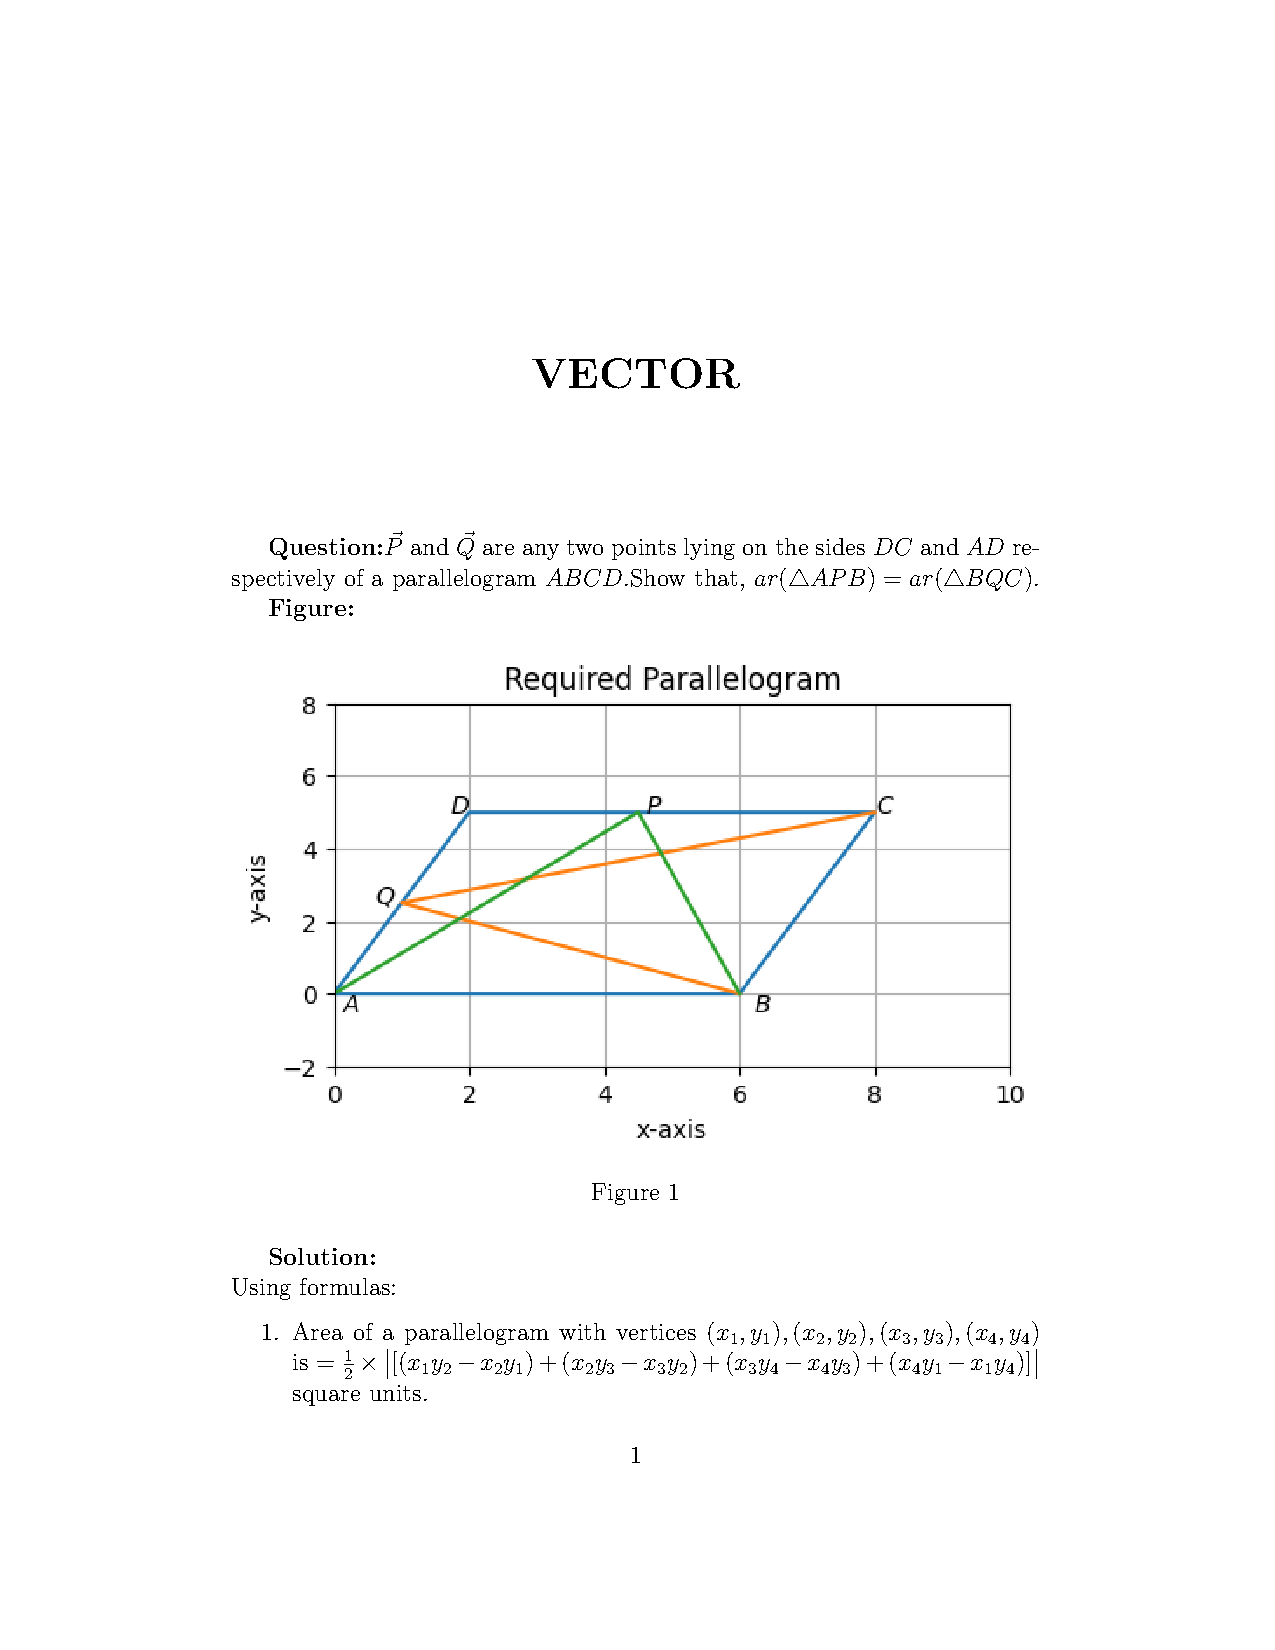
\includegraphics[width=\columnwidth]{fig/1.png}
    \caption{}
    \label{fig:fig:1}
\end{figure}


\textbf{Solution:}
\begin{table}[H]
   \centering
     \begin{tabular}{|c|c|c|}
    \hline
    \textbf{Input Parameters} &\textbf{Description} &\textbf{Value} \\
    \hline
     $\vec{O}$& Center(at origin)&$\vec{0}$\\
     \hline
 $r$ & Radius &1\\
 \hline
 $\theta$&-&$100\degree$\\
 \hline
 $\alpha$&-&$165.4\degree$\\
 \hline
 $\beta$&-&$5\degree$\\
 \hline
  \end{tabular}

   \caption{Table of input parameters}        
\label{tab:tab:1}                    
\end{table}




\begin{table}[H]
    \centering                                  
\begin{tabular}{|c|c|c|}
    \hline
        \textbf{Output Parameters} &\textbf{Description} &\textbf{Value} \\
\hline
          $\vec{Q}$ & Point &$\myvec{\cos{\theta_1}\\\sin{\theta_1}}$\\
          \hline
          $\vec{P}$ & Point &$\myvec{\cos{\theta_2}\\\sin{\theta_2}}$ \\
         \hline
          $\vec{R}$ & Point &$\myvec{\cos{\theta_3}\\sin{\theta_3}}$ \\
         \hline
    \end{tabular}

                  
\caption{Table of output parameters}
\label{tab:tab:2}
 \end{table}


For the $\triangle BQC$, the vertices of the triangle are taken from \tabref{tab:1} and \tabref{tab:2}.

\begin{align}
\implies ar\brak{\triangle BQC}&=
\frac{1}{2}\begin{tabular}{|c c c|}            
1 &1&1\\                      
$\vec{B}$&$\vec{Q}$&$\vec{C}$\\    
\end{tabular}\\
&= \frac{1}{2}\begin{tabular}{|c c c|}
       1 &1&1\\
       6&$\frac{2k_1}{k_1+1}$&8 \\
       0&$\frac{5k_1}{k_1+1}$&5
   \end{tabular}\\
  \xrightarrow{C_2'=C_2-C_1,C_3'=C_3-C_1}&\frac{1}{2} \begin{tabular}{|c c c|}
       1 &0&0\\
       6&$\frac{-4k_1-6}{k_1+1}$&2 \\
       0&$\frac{5k_1}{k_1+1}$&5
   \end{tabular}\\
&=\frac{1}{2}\brak{1\begin{tabular}{|c c|}
   $\frac{-4k_1-6}{k_1+1}$ &2  \\
   $\frac{5k_1}{k_1+1}$ & 5
\end{tabular} +0+0}\\
&=\frac{1}{2} \times30\\                          
&=15 \end{align}


For the $\triangle APB$, the vertices of the triangle are taken from \tabref{tab:1} and \tabref{tab:2}.
   \begin{align}
  \implies ar\brak{\triangle APB} &=
\frac{1}{2}\begin{tabular}{|c c c|}            
1 &1&1\\                            
$\vec{A}$&$\vec{P}$&$\vec{B}$\\
\end{tabular}\\ &=  \frac{1}{2}
   \begin{tabular}{|c c c|}
       1 &1&1\\
       0&$\frac{8k_2+2}{k_2+1}$&6 \\
       0&5&0
   \end{tabular}\\
 &=\frac{1}{2} \times30\\
 &=15 \end{align}
 \brak{6} = \brak{10}


So, ar\brak{\triangle BQC} = ar\brak{\triangle APB}.\brak{proved}
\end{document}

